\begin{enumerate}[label=\thesubsection.\arabic*, ref=\thesubsection.\theenumi]
	\item  Find the equation of the plane through the intersection of the planes $3{x} – {y} + 2{z} – 4 = 0 $ and $ {x} + {y} + {z} – 2 = 0$ and the point $\myvec{2\\2\\1}$.
		\label{prob:12/11/3/9/plane}
		\\
    \solution
		\begin{enumerate}[label=\thesubsection.\arabic*.,ref=\thesubsection.\theenumi]
	\item 
The intersection of the planes is given as
\begin{align}
	\label{eq:12/11/3/9/input}
\vec{n}_1^{\top}{\vec{x}} - {c}_1 + k\brak{\vec{n}_2^{\top}{\vec{x}} - {c}_2} &= 0
 \vec{n}_1 = \myvec{3\\-1\\2},\,
 \vec{n}_1 = \myvec{1\\1\\1},\,
	c_1 = 4, c_2 = 2.
\end{align}
\begin{align}
	\label{eq:12/11/3/9/eq}
\vec{n}_1^{\top}{\vec{x}} - {c}_1 + \lambda\brak{\vec{n}_2^{\top}{\vec{x}} - {c}_2} &= 0
\end{align}
where 
\begin{align}
	\label{eq:12/11/3/9/lam}
	\lambda = \frac{{c}_1 - \vec{n}_1^{\top}\vec{P}}{\vec{n}_2^{\top}\vec{P} - {c}_2} 
= -\frac{2}{3}  
\end{align}
upon substituting 
\begin{align}
\vec{P} = \myvec{2\\2\\1}.
\end{align}
	in \eqref{eq:12/11/3/9/lam} along with 
the numerical values in 
	\eqref{eq:12/11/3/9/input}.
	Now, substituting
	\eqref{eq:12/11/3/9/lam}
	in \eqref{eq:12/11/3/9/eq},
the equation of plane is 
\begin{align}
 \myvec{7&-5&4}\vec{x} = 8
\end{align}


\end{enumerate}

	\item  Find the equation of the line parallel to y-axis and drawn through the point of
intersection of the lines x – 7y + 5 = 0 and 3x + y = 0.
\\
\solution
		\begin{align}
	\myvec{3&-4}\vec{x}=\myvec{3&-4}\myvec{-2\\3}
	=-18 
\end{align}
is the required equation of the line.

    \item A person standing at the junction (crossing) of two straight paths 
    represented by the equations 
    \begin{align}
        \myvec{2&-3}\vec{x} = -4 
        \label{eq:chapters/11/10/4/24/L1}
    \end{align}
    and
    \begin{align}
        \myvec{3&4}\vec{x} = 5
        \label{eq:chapters/11/10/4/24/L2}
    \end{align} 
    wants to reach the path whose equation is 
    \begin{align}
        \myvec{6&-7}\vec{x} = -8
        \label{eq:chapters/11/10/4/24/L3}
    \end{align}
    Find equation of the path that he should follow.
\\
    \solution 
		\begin{align}
	\myvec{3&-4}\vec{x}=\myvec{3&-4}\myvec{-2\\3}
	=-18 
\end{align}
is the required equation of the line.

	\item Find the equation of the line passing through the point of intersection of the lines $4x + 7y - 3 = 0$ and $2x - 3y + 1 = 0$ that has equal intercepts on the axes.\\
	\solution 
	  		From \probref{prob:12/11/3/9/plane},
the intersection of the lines is given by 
		\begin{align}
       \myvec{4 + 2k &7-3k}\vec{x}=3-k
       \label{eq:11/10.4/12/3}
       \\
       \implies \myvec{4 + 2k \\7-3k} = \alpha\myvec{1 \\ 1} 
		\end{align}
			from  \probref{chapters/11/10/2/12}, yielding,
		\begin{align}
	\augvec{2}{1}{
				1 & -2 & 4
				\\
				1 & 3 & 7
			}
			\xleftrightarrow[]{R_2 = R_2 -R_1}
	\augvec{2}{1}{
				1 & -2 & 4
				\\
				0 & 5 & 3 
			}
			\\
			\text{or, } k = \frac{3}{5}
       \label{eq:11/10.4/12/4}
   \end{align}
 Substituting the above  
in       \eqref{eq:11/10.4/12/3}, the desired equation is 
    \begin{align}
        \myvec{1&1}\vec{x}=\frac{6}{13}
    \end{align}
    See
    \figref{fig:enter-label}.
\begin{figure}[H]
    \centering
    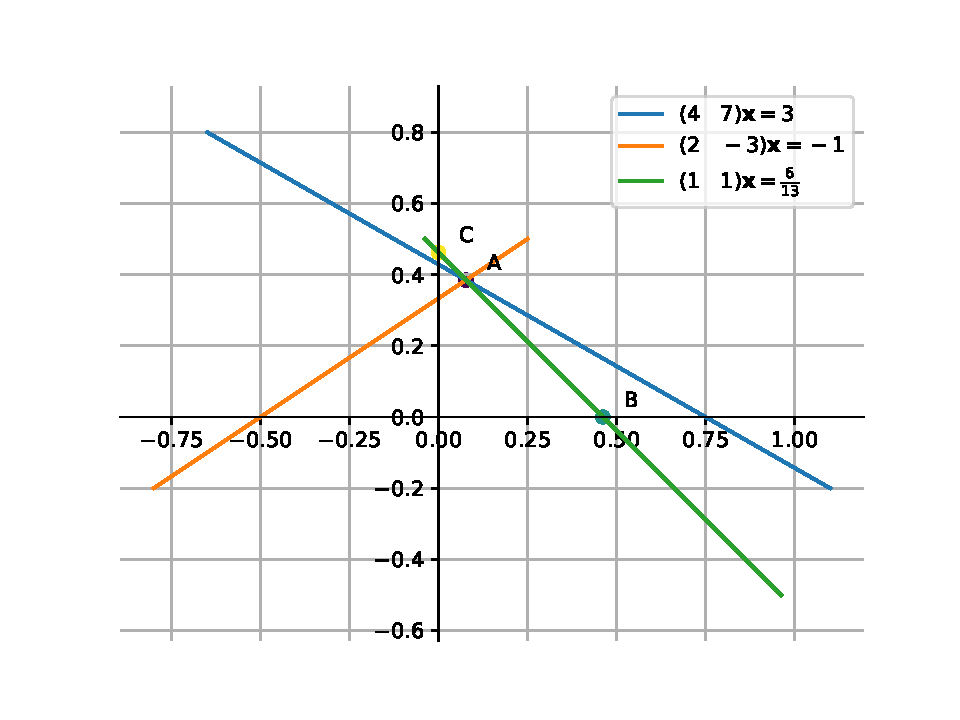
\includegraphics[width=0.75\columnwidth]{chapters/11/10/4/12/figs/fig.pdf}
    \caption{}
    \label{fig:enter-label}
\end{figure}

\item
Find the value of $p$ so that the three lines $3x+y-2=0,  px+2y-3=0$ and $2x-y-3=0$ may intersect at one point.
\label{11.10.4.9}
\\
\solution
Performing row operations
on the matrix
\begin{align*}  
\myvec{
    3 &1&-2 \\
     p&2&-3\\
     2&-1&-3
}
\xrightarrow[R_3=3R_3-2R_1]{R_2=3R_2-pR_1}&\myvec{
    3&1&-2\\
     $0$&6-p&-9+2p\\
     0&-5&-5}\\
 \xrightarrow{R_3=R_3(6-p)+5R_2}&\myvec{
    3&1&-2\\
     0&6-p&-9+2p\\
     0&0&-75+15p}
     \\
  \implies 
    p=5
\end{align*}
Substituting this value in the above, we obtain
\begin{align}
\myvec{
    3&1&-2\\
     0&1&1\\
     0&0&0}
\end{align}
yielding
\begin{align}
	\vec{x} = \myvec{-1 \\ 1}
\end{align}
as the point of intersection.
    See \figref{fig:11.10.4.9}.
\begin{figure}[H]
    \centering
    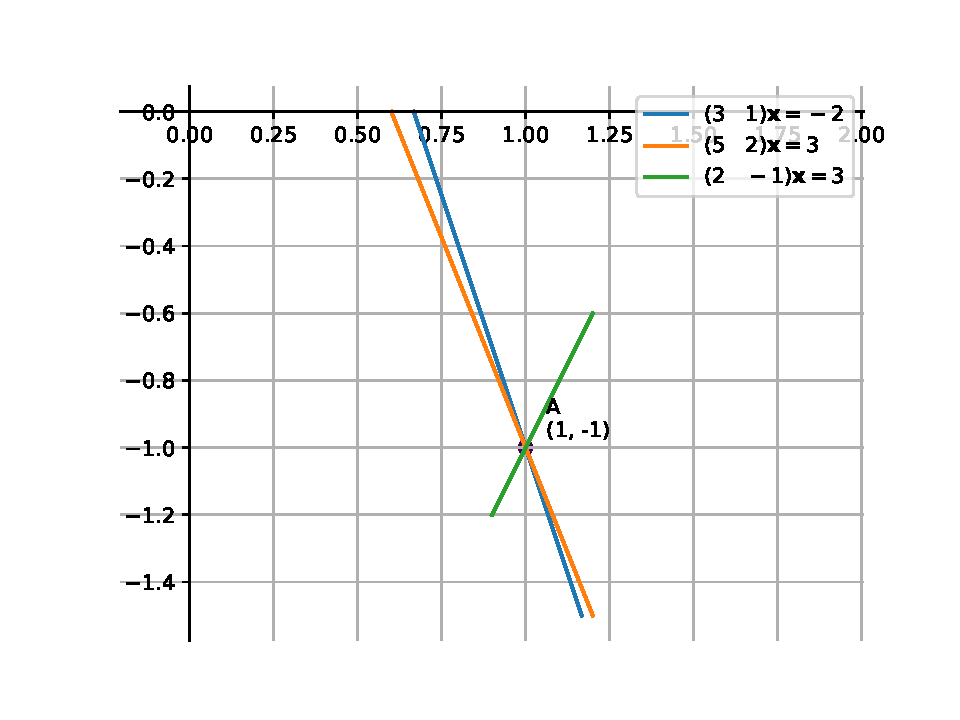
\includegraphics[width=0.75\columnwidth]{chapters/11/10/4/9/figs/fig.pdf}
    \caption{}
    \label{fig:11.10.4.9}
\end{figure}


\item Show that the lines
$$\frac{x-1}{2}=\frac{y-2}{3}=\frac{z-3}{4}$$
 and 
$$ \frac{x-4}{5}=\frac{y-1}{2}=z  $$
 intersect.
 Also,  find their point of intersection.
\item The area of the region bounded by the curve $y = x + 1$ and the lines $x = 2$ and $x = 3$ is
	\begin{enumerate}[itemsep=1ex]
\item $\frac{7}{2}$ sq units
\item $\frac{9}{2}$ sq units
\item $\frac{11}{2}$ sq units
\item $\frac{13}{2}$ sq units
\end{enumerate}   
\item Compute the area bounded by the line $x + 2y = 2$,  $y - x = 1$ and $2x + y = 7$.
\item Find the area bounded by the lines $y = 4x + 5$,  $y = 5 - x$ and $4y = x + 5$.
\item Find the equation of the plane which is perpendicular to the plane $5x+3y+6z+8=0$ and which contains the line of intersection of the planes $x+2y+3z-4=0$ and $2x+y-z+5=0.$
\item  Point $\vec{P}(0, 2)$ is the point of intersection of the $y$-axis and the perpendicular bisector of line segment joining the points $\vec{A}(-1, 1) $ and $ \vec{B}(3, 3)$.
\item Prove that the line through $\vec{A}(0, -1, -1)$ and $\vec{B}(4, 5, 1)$ intersects the line through $\vec{C}(3, 9, 4)$ and $\vec{D}(-4, 4, 4)$.
\item Find the equation of the plane through the intersection of the planes $\overrightarrow{r} \cdot (\hat{i}+3\hat{j}) - 6=0$ and $\overrightarrow{r} \cdot (3\hat{i}-\hat{j}-4\hat{k})=0, $ whose perpendicular distance from origin is unity.
\item Find the equation of the line passing through the point of intersection of $2x+y=5$ and $x+3y+8=0$ and parallel to the line $3x+4y=7$.
\item Find the equations of the lines through the point of intersection of the line $x-y+1=0 $ and $2x-3y+5=0$ and whose distance from the point (3, 2) is $\frac{7}{5}$.
\item The straight line $5x+4y=0$ passes through the point of intersection of the straight lines $x+2y-10=0$ and $2x+y+5=0$.
\item Find the equation of the plane passing through the line of intersection of the planes  $\overrightarrow{r}\cdot(\hat{i}+\hat{j}+\hat{k})=1$ and $\overrightarrow{r}\cdot(2\hat{i}+3\hat{j}-\hat{k})+4=0$ and parallel to the $X$ axis.
\item Find the equation of the plane which contains the line of intersection of the planes $\overrightarrow{r}\cdot(\hat{i}+2\hat{j}+3\hat{k})-4=0,  \overrightarrow{r} \cdot  (2\hat{i}+\hat{j}-\hat{k})+5=0$ and which is perpendicular to the plane $\overrightarrow{r}\cdot(5\hat{i}+3\hat{j}-6\hat{k})+8=0$
\item Find the distance of the point $(-1, -5, -10)$ from the point of intersection of the line $\overrightarrow{r}=2\hat{i}-\hat{j}-2\hat{k}+\lambda(3\hat{i}+4\hat{j}+2\hat{k})$ and the plane $\overrightarrow{r}\cdot(\hat{i}-\hat{j}+\hat{k})=5$.
\item Show that the area of the triangle formed by the lines $y=m_1x+c_1,  y=m_2x+c_2$ and $x=0$ is $\frac{\brak{c_1-c_2}^2}{2\abs{m_1-m_2}}$
\item If the lines $2x+y-3=0,  5x+ky-3=0$ and $3x-y-2=0$ are concurrent,  find the value of $k$.
\item Find the vector equation of the plane passing through the intersection of the planes $\overrightarrow{r} \cdot (\hat{i} +\hat{j} +\hat{k})=6$ and $\overrightarrow{r} \cdot (2\hat{i} +3\hat{j} +4\hat{k})=-5$,  and the point $(1,  1,  1)$.
\item Find the coordinates of the point where the line through the points $\vec{A}(3, 4, 1)$ and $\vec{B}(5,  1,  6)$ crosses the $XY$ plane.
\end{enumerate}
